\documentclass[twocolumn,a4paper, 10pts]{article}
\usepackage[utf8]{inputenc}
\usepackage[english]{babel}
\usepackage[T1]{fontenc}
\usepackage{amsmath}
\usepackage{bm}
\usepackage{braket}
\usepackage{amssymb}
\usepackage{float}
\usepackage{fancyhdr}
\usepackage{lastpage}
\usepackage{appendix}
\usepackage{breqn}
\usepackage{gensymb}
\usepackage{xfrac}
\usepackage{listings}
\usepackage{caption}
\usepackage{subcaption}
\usepackage{wrapfig}
\usepackage{lipsum}
\usepackage{multicol}
\usepackage{svg}
\usepackage{newclude}
\usepackage{hyperref}

\pagenumbering{gobble} 

%%% Margins
\usepackage[a4paper,left=0.5in,right=0.5in,top=0.5in,bottom=0.5in]{geometry}

\lstset{language=[Sharp]C}

\begin{document}
\title{\vspace{-1.7cm}Exam Project - Symmetric Rank-1 Update Method}
\author{Mads Hansen Baattrup - \href{https://github.com/mads-hb/ppnm-2022}{\textbf{Repository}}}
\maketitle

\section*{Problem}
The two last digits in my student number are $76$ which means that I have solved problem $76\%23=7$, which is called 'Symmetric rank-1 update of a size-n symmetric eigenvalue problem'. The problem is concerned with finding the eigenvalues of a matrix, $\mathbf{A}$:

\begin{align}
\label{eqn:matrix-system}
\mathbf{A}=\mathbf{D}+\sigma \mathbf{u}\mathbf{u}^\intercal,
\end{align}

where $\mathbf{D}$ is a diagonal matrix, $\mathbf{u}$ is a column vector, and $\sigma$ is some real number. The problem of finding eigenvalues of $\mathbf{A}$ can be solved in $O(n^2)$ time.

\section*{Solution}
The secular equation describing the eigenvalues of a matrix system of the form in eqn. \ref{eqn:matrix-system} is:
\begin{align}
1+\sum_{i=1}^m\frac{\sigma u_i^2}{D_{ii}-\lambda_i}=0,
\end{align}
where $m$ is the number of non-zero components of the update vector, $\mathbf{u}$ and $\lambda_i$ is the $i$'th eigenvalue. The roots of the secular equation can be found using the Newton-Raphson method. In the implementation I have made here, I have found the eigenvalues sequentially for numerical stability, since I found that the root-finding over a large vector was unstable. Furthermore, I have computed the Jacobian of the system using finite differences instead of using the analytical Jacobian. This is because the analytical Jacobian did not provide any speed-up compared to the Jacobian based on finite differences.
\par
The spectrum of eigenvalues found by this symmetric rank-1 update method is compared to the spectrum found by the Jacobi diagonalization routine. The results of such a comparison are shown in figure \ref{fig:spectrum} for a random $10\times 10$ matrix. As can be seen, the eigenvalues are equal - or very close to being equal at least. Any numerical difference is expected to come from the relative error in the root-finding method.
\begin{figure}[h]
    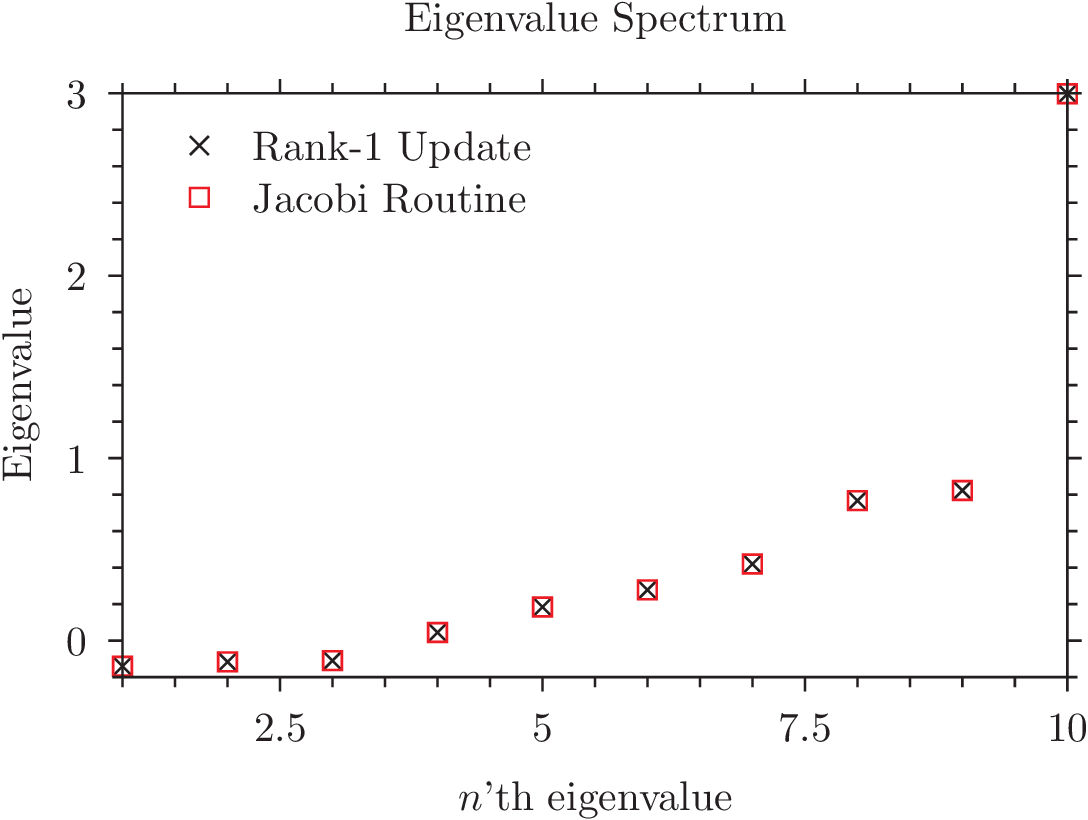
\includegraphics[width=0.48\textwidth]{img/eig_spectrum.png}
    \caption{Spectrum of eigenvalues for a random matrix system of the form as described in eqn. \ref{eqn:matrix-system}. The eigenvalues are found by the symmetric rank-1 update method and by a Jacobi diagonalization routine.}
    \label{fig:spectrum}
\end{figure}
\par
It is also shown that the time complexity of the symmetric rank-1 update method is $O(n^2)$ as opposed to the $O(n^3)$ time complexity of the Jacobi diagonalization routine. Figure \ref{fig:timing} shows the time complexity as a function of the dimensionality of the matrix. I have used the least squares method implemented earlier in the course to show that the time complexities are $O(n^2)$ and $O(n^3)$ respectively.
\par
The rank-1 update method is found to have some numerical instabilities clearly evident in figure \ref{fig:timing} as bumps in the data. These are places where the eigenvalues did not converge within the maximum number of iterations tolerated in the root-finding method. This also means that the computed eigenvalues of these matrices do not perfectly correspond to the eigenvalues found by a Jacobi diagonalization routine. I think a likely explanation of this is that the root-finding method requires initial parameters, and especially the initial guesses outside the eigenvalue spectrum of $\mathbf{D}$ are prone to being very wrong.
\begin{figure}[h]
    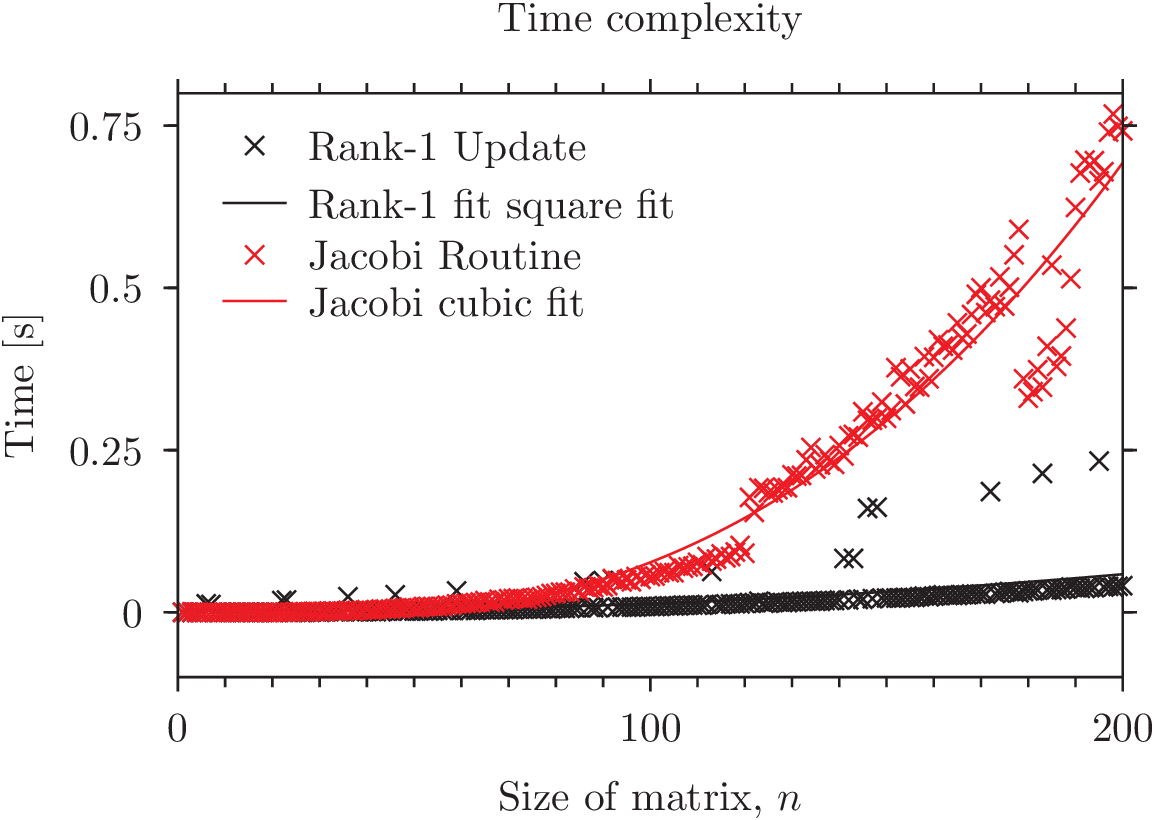
\includegraphics[width=0.48\textwidth]{img/timing.png}
    \caption{Time complexity of the symmetric rank-1 update method and the Jacobi diagonalization routine. Spectrum is generated by generating random matrix system of size $n$ and then finding the eigenvalues of these random matrices. Please note that the symmetric rank-1 method has been fitted to a polynomial of order two and the Jacobi diagonalization routine has been fitted to a polynomial of order three.}
    \label{fig:timing}
\end{figure}

\end{document}